\section{Complementary Techniques - Trace and Parameters Analysis as \mas support}\label{sec:complementary}
\textcolor{blue}{All this section is new for TSE journal...}

Our work, although closely related to previous studies, differs from them in several aspects.  First, our assessment is more comprehensive: instead of considering $102$ pairs of benign/malign apps, we execute our study considering \apps pairs of apps. We then investigate which characteristics of the malware samples in the large dataset explain the lower performance. We observed and also explore two extensions to the \mas. First we compare the traces from the app entry points to the calls to sensitive APIs, and second we replicate the additional verification proposed by Le et al.~\cite{le2018towards}, that observed the values of the parameters used in the calls to sensitive API. In the end, we checked the accuracy of these extension at a more representative dataSet.

Regarding trace analysis, we build the dynamic call graphs that characterize the execution of each version of the apps in our dataset. Our goal is to explore how many pairs of apps call the same set of sensitive APIs, though using different call traces. We hypothesize that differences in the traces might be used to complement the \mas for suspicious app identification. As such, here we execute the trace analysis for all app pairs of our dataset, and check if there are situations in which the basic version of the \mas was not able to correctly classify the malign version of an app as a piggybacked, however it has a different execution trace. For detecting different trace, we performed an evaluation of the dynamic call graph of each pair. Our procedure checks if there is some new node, representing a new sensitive API at malicious version, or a new edge($x$, $y$), where $x$ and $y$ indicates a method $x$ calling a sensitive method $y$. Figure~\ref{fig:callGraph} illustrates an example of benign and malicious call graphs.
At this example, although both app versions access the same set of sensitive resources, the
malicious version follows a different execution trace. 


\begin{figure}[ht]
\centering
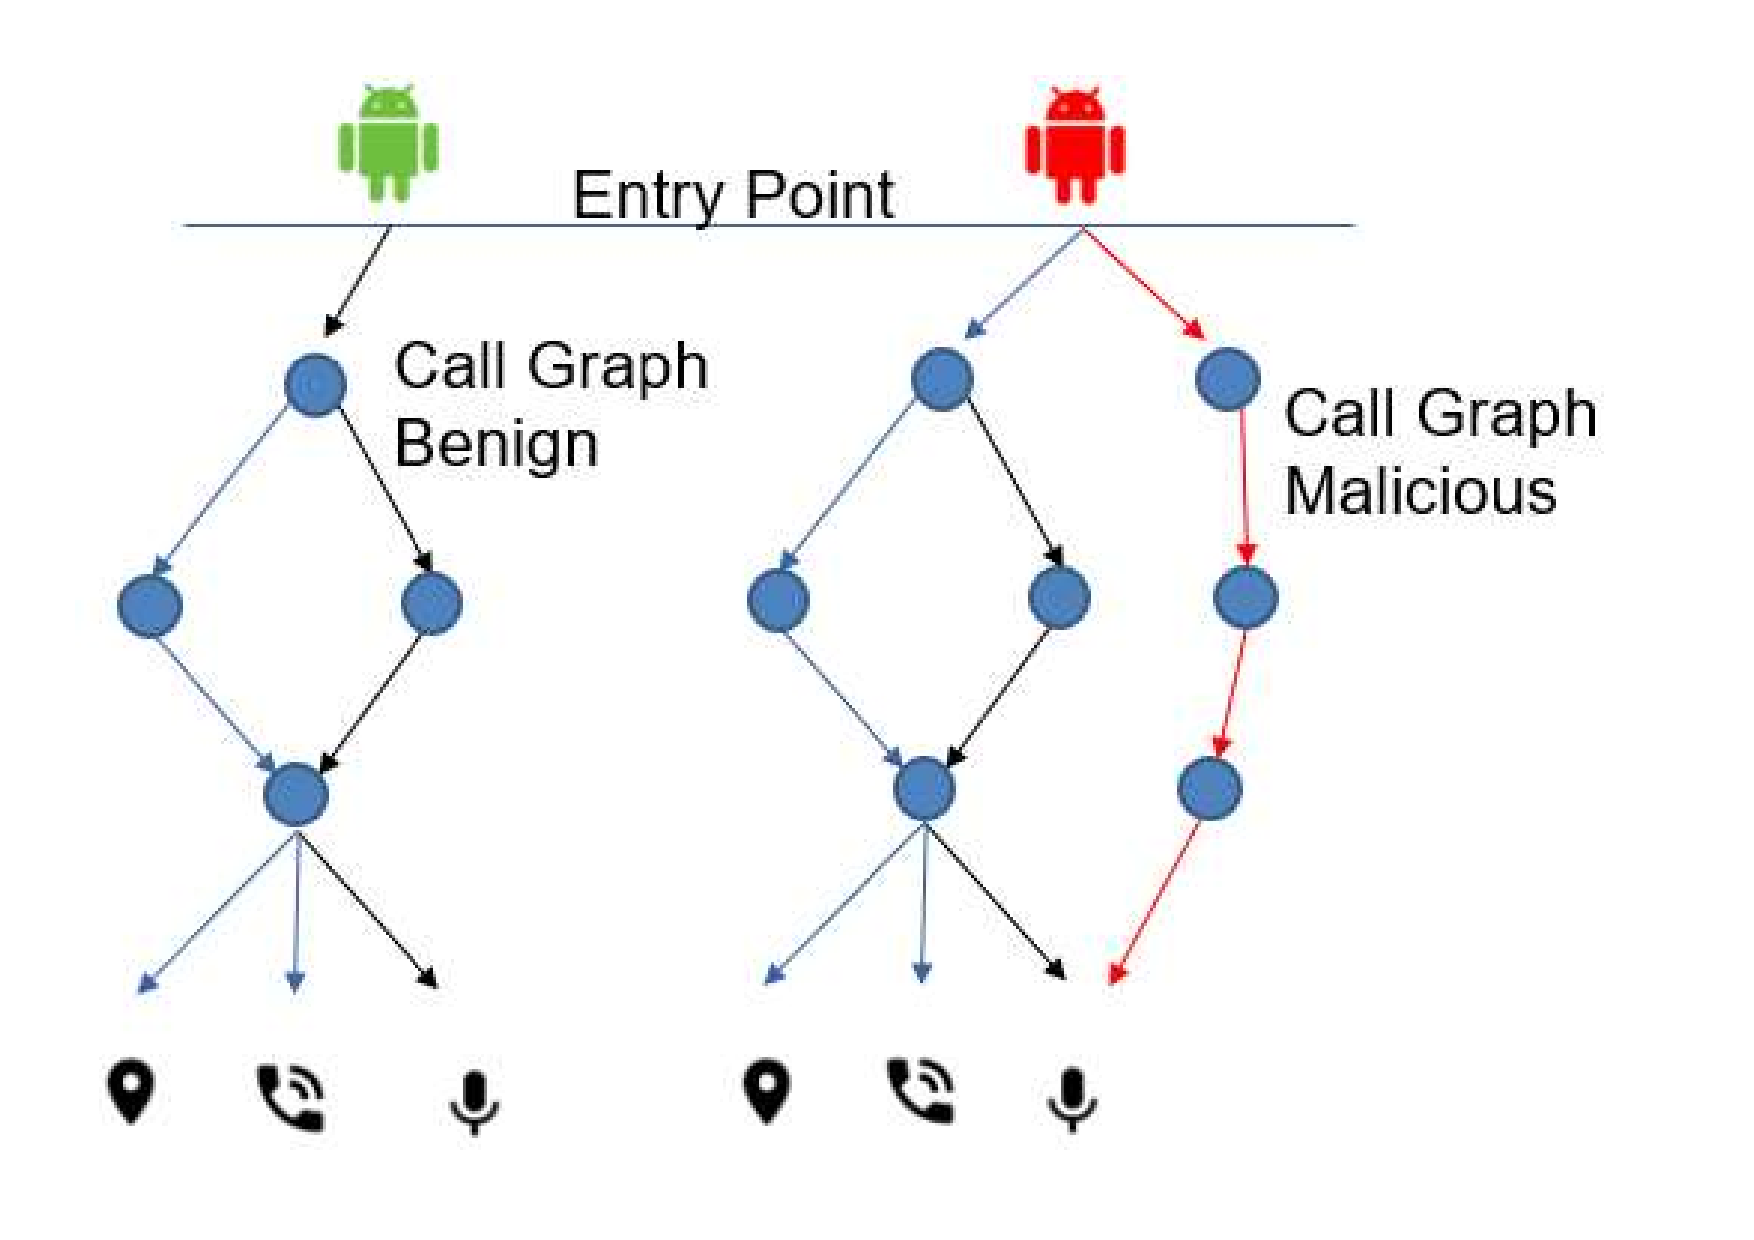
\includegraphics[scale=0.30]{images/maliciousCallGraph.pdf}
\caption{Illustrative example of the trace analysis. In this case, both versions call the same set of sensitive APIs. Nonetheless,
the traces between the entry point and the calls to sensitive APIs diverge.}
 \label{fig:callGraph}
\end{figure}

\begin{figure}
\centering
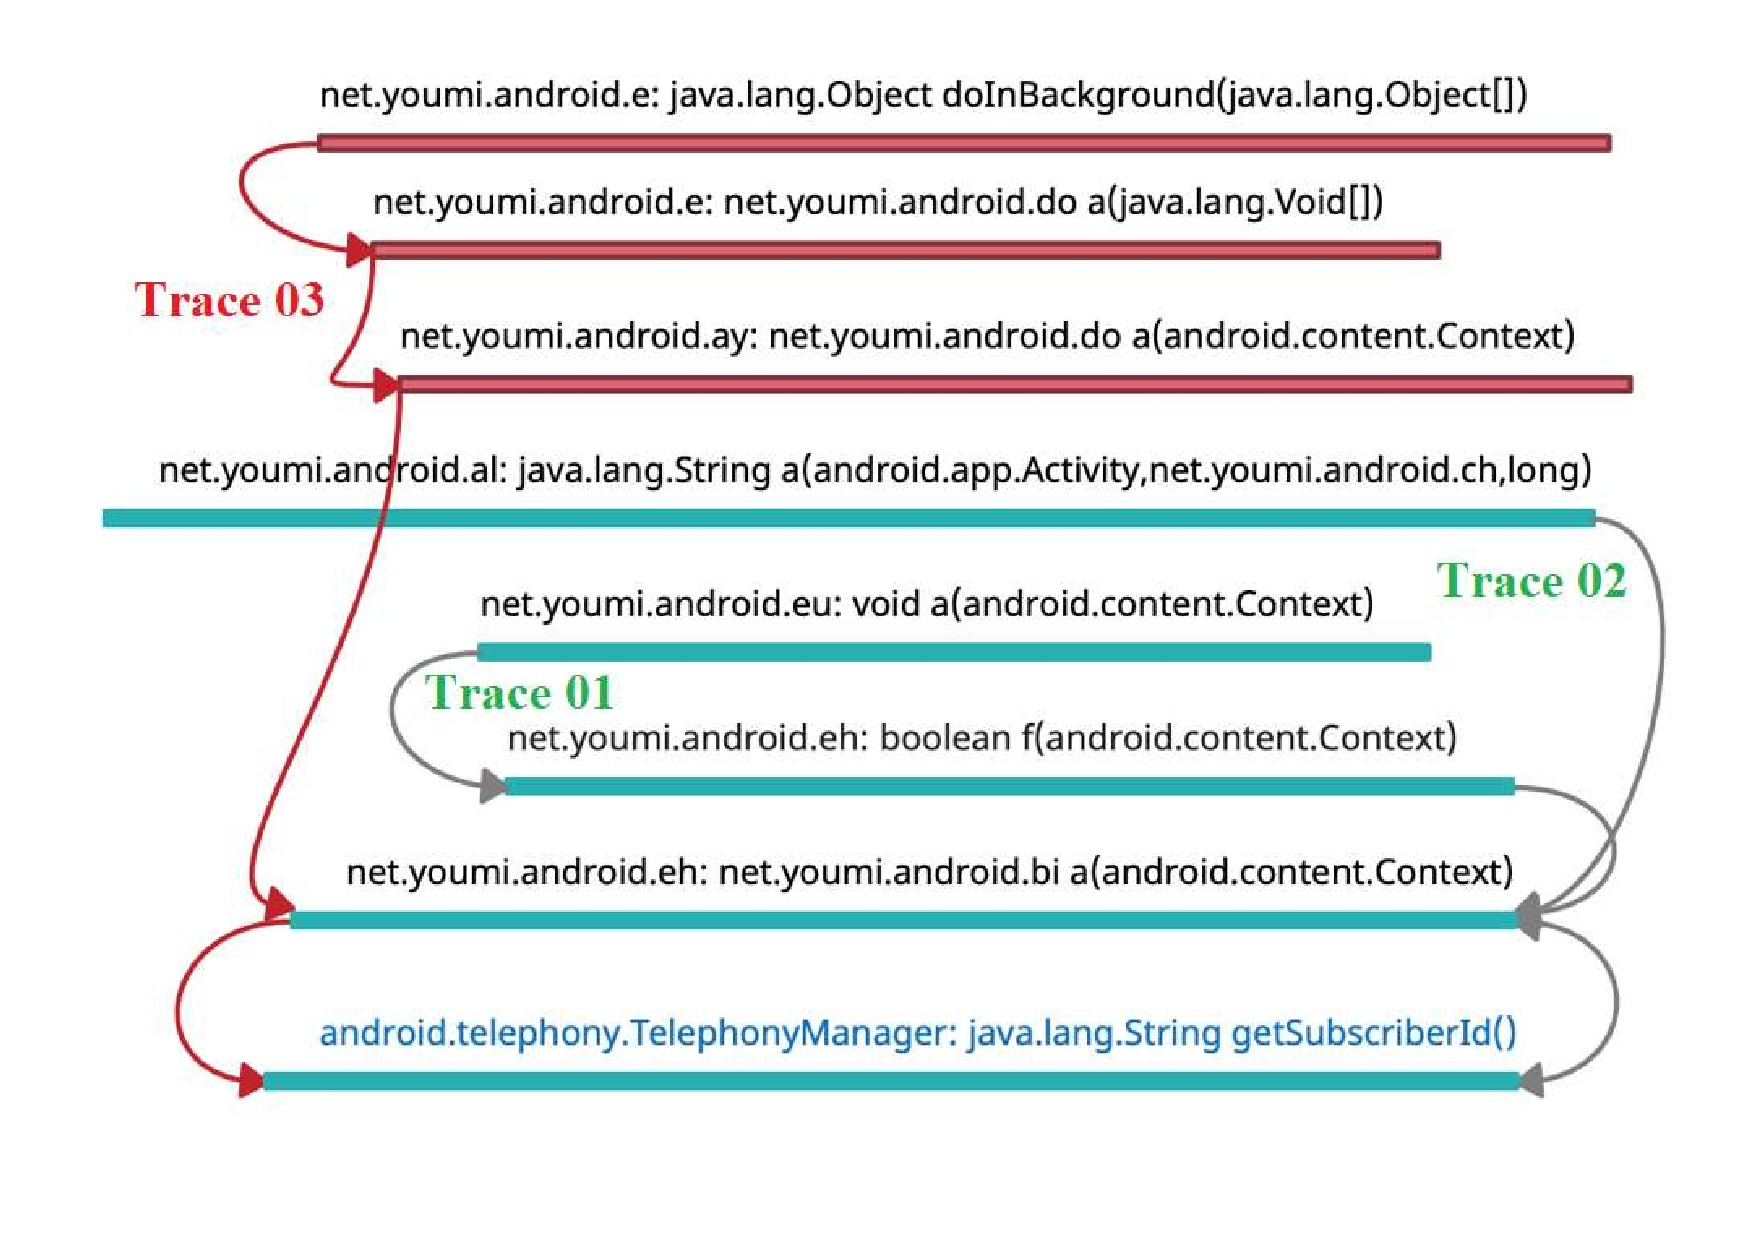
\includegraphics[scale=0.28]{images/maliciousTrace_example01.pdf}
\caption{Example of Malicious Trace.}
 \label{fig:maliciousTrace}
\end{figure}


Figure~\ref{fig:maliciousTrace} shows an example of a trace injected in the malicious version of the
app \textbf{[com.android.remotecontrolppt]}. Here, the benign and malicious app versions access the same
sensitive method, \textit{getSubscriberid()}. This sensitive method returns the device's unique
subscriber ID, and requires the manifest file permission \texttt{READ\_PHONE\_STATE}, present in both app versions.
The original app accesses this method through two distinct traces (Trace 01 and Trace 02), which suggests an expected action from app user. However,
instead of the two original traces, the malicious version injected a third trace (Trace 03) containing as entry point a method that performs a stealth
computation on a background thread, \textit{doInBackground}, suggesting an action without user's awareness.

As described at~\cite{le2018towards}, malicious apps may require external data, like a remote server address to push an advertisement, or sink sensitive information to another location, different from the original, using SMS message for example. For this purpose, malicious apps may insert parameter to a sensitive APIs, different from the original app. Thus, we also hypothesize that differences parameter (from both app version), passed to the same sensitive APIS, may provides hints for suspicious repackaged apps. Figure~\ref{fig:parameterDiff} presents an example of different parameters inserted at the same method, extracted from monitored \textit{logcat}. This example just use a \textit{java.net.URL} object to present a different advertising from the original app. Although not expressly harmful, repackaged app may uses objects from this \textit{Class} to download and run external files from a network in the infected system\cite{DBLP:journals/compsec/ObaidatSPP22}.



\begin{figure*}[t]
\centering
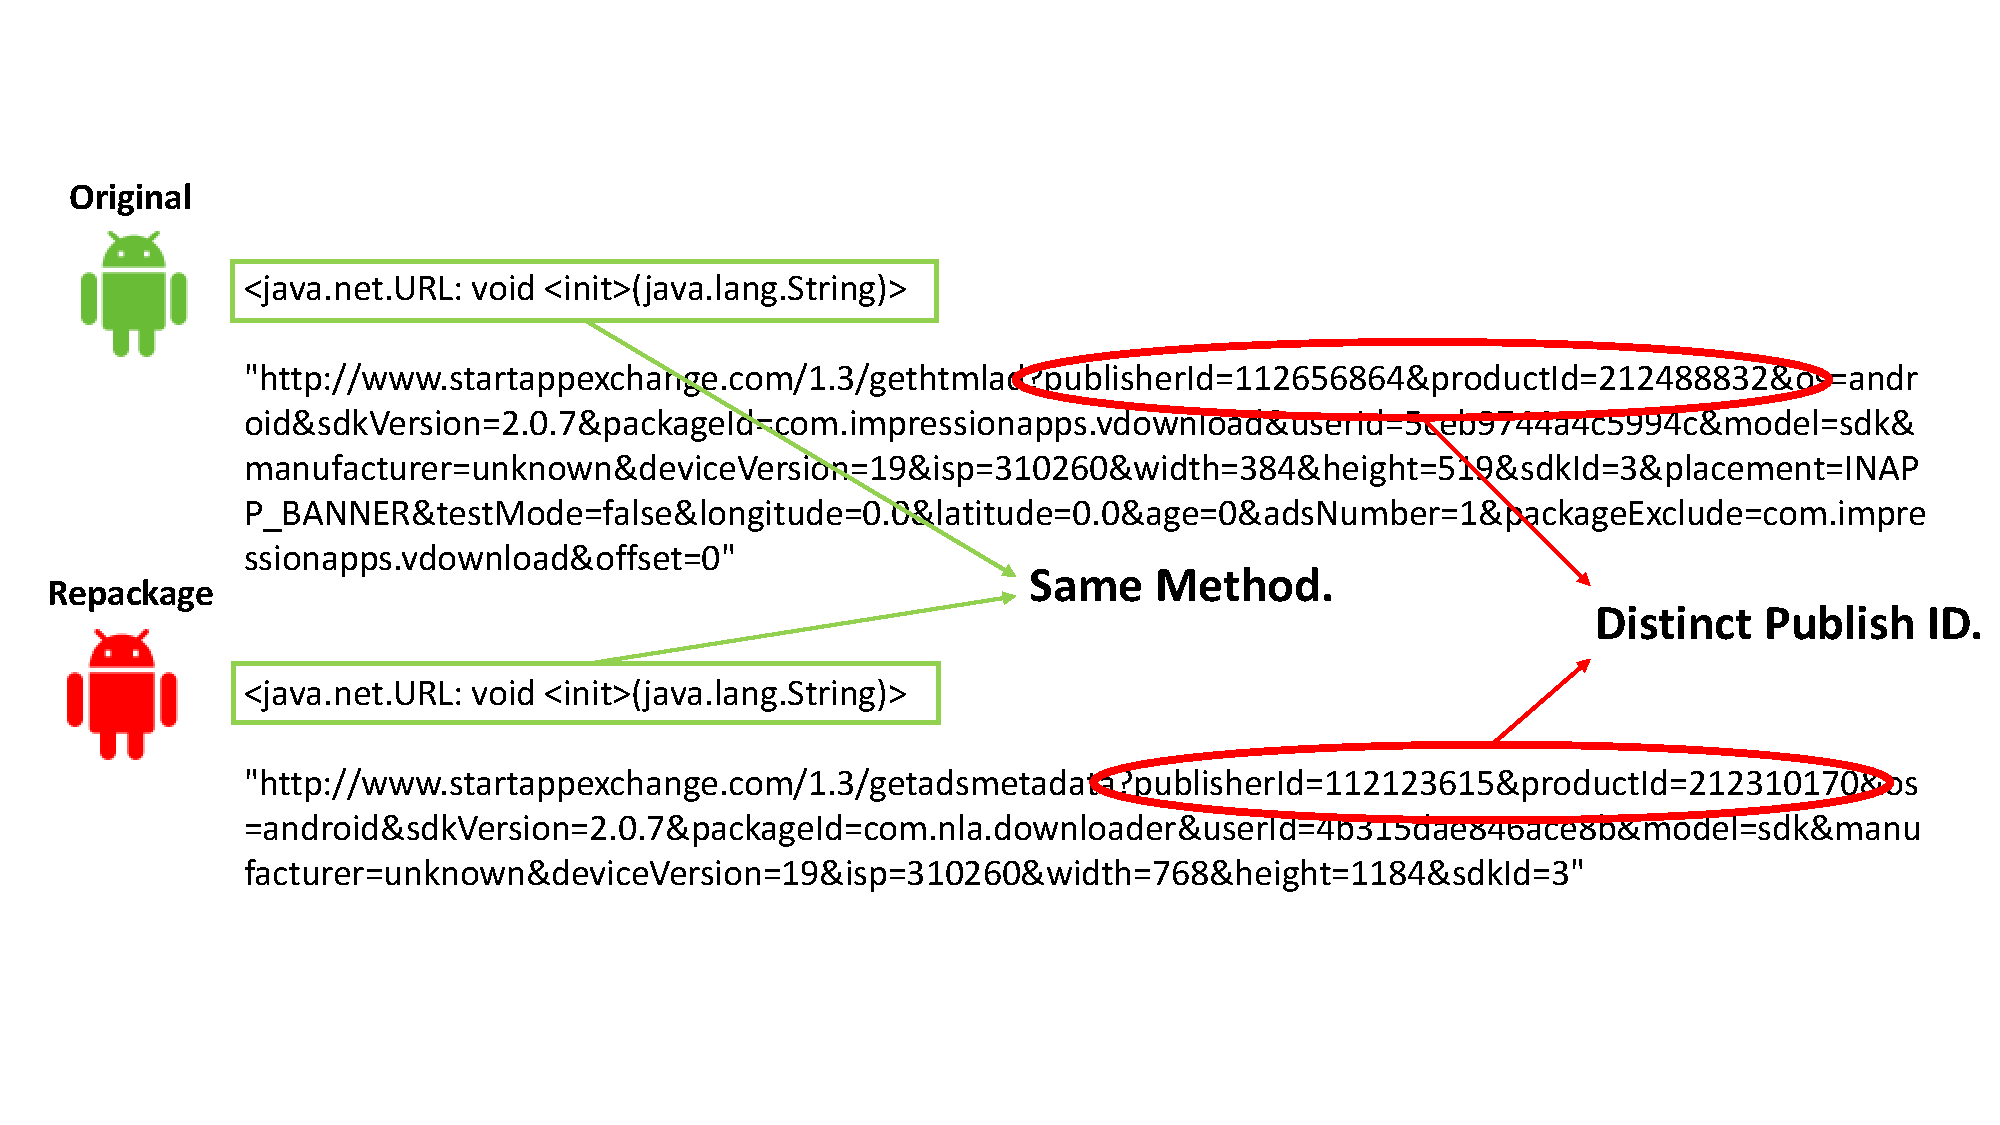
\includegraphics[scale=0.3]{images/parameterDiff.pdf}
\caption{Example of different parameters inserted at the same method.}
 \label{fig:parameterDiff}
\end{figure*}